%\documentclass[12pt]{article}
\documentclass[draft,jgrga]{AGUTeX}
\usepackage{amsmath}
\usepackage[dvips]{graphicx}
\usepackage{xcolor}

\authorrunninghead{ZHENG ET AL.}
\titlerunninghead{DNS for Entrainment}

\newcommand{\Eq}[1]{Eq.~\eqref{#1}} \newcommand{\Fig}[1]{Figure~\ref{#1}}
\newcommand{\Sec}[1]{Sec.~\ref{#1}} \newcommand{\Table}[1]{Table~\ref{#1}}

\begin{document}
\title{A New Particle-Resolved Direct Numerical Simulation Model for Studying Entrainment Processes}
\author{Zheng Gao,\altaffilmark{1}
Yangang Liu,\altaffilmark{2}
Xiaolin Li,\altaffilmark{1}}

\altaffiltext{1}{Department of Applied Mathematics and Statistics, Stony Brook University,
Stony Brook, NY 11794--3600, USA.}
\altaffiltext{2}{Brookhaven National Laboratory, Bldg. 815E Upton, NY 11973-5000}

\begin{abstract}
A new particle-resolved three dimensional direct numerical simulation (DNS) model is developed that combines Lagrangian droplet tracking with the Eulerian field representation. Different initial settings in the decaying and forced turbulence environments are simulated to investigate the processes of entrainment of clear air and its mixing with cloudy air and their interactions with cloud microphysics.
The results show that even with the same cloud water fraction, the thermodynamic and microphysical properties are highly different with different settings, especially for the decaying cases. The results suggest that the initial shape of cloud filaments should be considered as a significant factor in the study of cloud entrainment and mixing.   
\end{abstract}

\begin{article}

\section{Introduction}
The microphysics of cloud droplets in small-scale, such as evaporation and condensation add some uncertainties to the Large-eddy simulation (LES) models \cite{Jarecka13}, by impacting on the spectrum of cloud droplets during entrainment and mixing process. It was poorly understood that whether the reduction of liquid water content was through the reduction of only the droplet size (extremely homogeneous mixing), or only the number of droplets (extremely inhomogeneous mixing), or both the number and size (inhomogeneous mixing). These situations are defined by comparing two time scales: the turbulent homogenization time scale and droplet evaporation time scale. In the extreme cases, one time scale will dominate the other while in the unextreme case the two scales are comparable. Recently, it has been demonstrated that different mixing scenarios can occur and change during one single cloud evolution (\cite{And09,Burnet07,Lehmann09}). Therefore, it becomes more and more important to have a reasonable and accurate estimation of the mixing scenario for a sub-grid model. \cite{Jarecka2013}, utilized the DNS results from \cite{And04,And06,And09}  to estimate the mixing scenario with a parameter $\alpha$ and successfully merged the $\lambda$-$\beta$ subgrid scheme (\cite{Jarecka2009}) with the double-moment LES model(\cite{Morrison2008}). \cite{Lu2013}, proposed the transition scale number to measure the occurrence probability of homogeneous or inhomogeneous entrainment-mixing process. Both of the cloud observations and numerical simulations imply a positive relationship between the transition scale number and the homogeneous mixing degree. In spite of many progresses in the study of cloud microphysics, to capture the details of turbulent transportation and dilution of cloud water is still a challenge for representing clouds in coarse-resolution climate model.
   
As a supplementary to laboratory experiments (e.g., \cite{Malinowski1998}), DNS allows extracting information that is difficult to obtain in the laboratory. In specific, DNS gives a complete view of the mixing process at various length scales from energy containing scale to dissipation length scale.
It is also efficient to study the correlation of two different variables by changing the parameters of the simulator. In the past decades, many authors have contributed to the DNS
of entrainment and mixing processes. In Andrejczuk and Grabowski's series work \cite{And04,And06,And09}, an incompressible Boussinesq approximation model, along with vapor mixing ratio and temperature, is proposed to study the cloud-clear air interfacial mixing. Different turbulence kinetic energy (TKE) are used as input parameters at initial time to examine the impact of turbulence intensity on droplet size distribution and mixing homogeneity. The cloud filaments and velocity field are preset to make a heavily idealized initial and boundary condition, while focusing on the details of the evolving flow. 

Kumar and Schumacher in \cite{Kumar11,Kumar12} developed a particle-point DNS to investigate entrainment mixing processes. In their work, a slab-like vapor field is adopted to mimic the supersaturated cloud area and subsaturated environment. The effects of temperature and buoyancy are ignored while an artificial isotropic volume forcing is introduced to maintain the turbulence. Using isotropic artificial forced turbulence is valid for adiabatic cloudy areas, but might be unrealistic at the interface between cloudy and clear air, because the flow in the regions of mixing may not be isotropic due to the negative buoyancy from the droplet evaporation \cite{Vaillancourt00}. In \cite{Kumar14}, the authors extended their previous work to both forced and decaying turbulence, and claimed that the buoyancy due to droplet evaporation played minor role in the mixing for their configuration.

It is interesting to notice that the models and settings in \cite{Kumar11} and \cite{And04} are similar except the geometric shape of the cloud filaments. The cloudy area in \cite{And04} is completely decided by the velocity field of the turbulent flow, thus forming worm-like regions, while a slab-like cloud filament is adopted in \cite{Kumar11}. Since no particular reasons of their choices are given and the effects of cloud shape on the mixing processes are unknown, an investigation on the settings of cloud filaments in DNS becomes significant. In this paper, three different cloud shapes, including the ones in \cite{Kumar11} and \cite{And04}, are tested in the simulation.

The rest of the paper is organized as follows. Section 2 describes
the mathematics model and numerical scheme. In section 3, we give
a brief introduction to the procedure of setting up initial state for simulation. The numerical results and some post-analysis are shown
in section 4. A summary is presented in the last section. 
\section{Particle-Resolved DNS}


\subsection{Dynamical and scalar field}

Following previous DNS, the new DNS is based on the incompressible
Boussinesq approximation whereby the dynamical field is by \cite{And04}:

\begin{subequations}

\begin{equation}
\partial_{t}\mathbf{u}+(\mathbf{u}\cdot\nabla)\mathbf{u}=-\frac{1}{\rho_{0}}\nabla p+\nu\nabla^2 \mathbf{u}+\mathbf{f}_b + \mathbf{f}_e\label{eq:NS1}
\end{equation}


\begin{equation}
\nabla\cdot \mathbf{u}=0\label{eq:NS2}
\end{equation}

\end{subequations}

where $\nu$ is the kinetic viscosity, $\rho_{0}$ is the density of
dry air, $\mathbf{u}$ is the velocity field, $p$ is the pressure field. Here $\mathbf{f}_b$ is the force immitating the buoyancy effects and $\mathbf{f}_e$ is the external low-wavenumber forcing:
\begin{equation}
\mathbf{f}_b= 
-\mathbf{g}[\frac{T-T_{0}}{T_0}+0.608(q_{v}-q_{v0})-q_{c}]
\label{eq:source_term}
\end{equation}
where $\mathbf{g}$ is the gravity, $T$ and $q_{v}$ are temperature
and vapor mixing ratio field respectively with the subscript ``$0$''
denoting the reference values; $q_{c}$ is the cloud water mixing
ratio. $\mathbf{f}_e$ is the artificial external force defined in the Fourier space:
\begin{equation}
\mathbf{f}_e = \epsilon_{in}\frac{\mathbf{u}(\mathbf{k},t)}
{\sum_{\mathbf{k}_f\in \kappa}|\mathbf{u}(\mathbf{k}_f,t)|^2}
\sigma_{\mathbf{k},\mathbf{k}_f}
\end{equation}
where $\mathbf{k}$ is chosen from a subset of the wavenumber space $\kappa$ containing a few wavevectors, $\epsilon_{in}$ is the input energy rate. $\delta_{k,k_f}$ is a delta function. Therefore, statistics stationary homogeneous turbulence 
can be obtained in DNS by forcing the low-wavenumber modes.

The temperature and vapor mixing ratio are solved from the following
equations (\cite{Kumar11}):

\begin{equation}
\partial_{t}T+(\mathbf{u}\cdot\nabla)T=\frac{L_{h}}{c_{p}}C_{d}+\mu_{T}\nabla^{2}T\label{eq:Temp}
\end{equation}
\begin{equation}
\partial_{t}q_{v}+(\mathbf{u}\cdot\nabla)q_{v}=-C_{d}+\mu_{v}\nabla^{2}q_{v}\label{eq:Vapor}
\end{equation}


In the above equations, $L_{h}$ is the latent heat of water vapor condensation,
$c_{p}$ is the specific heat at constant pressure, $\mu_{T}=\mu_{v}$ are
the molecular diffusivity for temperature and water vapor, respectively
and assumes to be equal. The condensation rate $C_{d}$ is defined as the rate of exchanging water between liquid and vapor per unit time, and is described by:

\begin{subequations}

\begin{equation}
C_{d}(\mathbf{X},t)=\frac{d(m_{l}(\mathbf{X},t))}{m_{a}dt}=\frac{4\pi\rho_{l}K}{\rho_{0}a^{3}}\Sigma_{i=1}^{n}S(\mathbf{X}_{i},t)R_{i}(t)\label{eq:CondRate}
\end{equation}


where $K$ is a function of temperature and pressure given by:

\begin{equation}
K=1/[(\frac{L_{h}}{R_{v}T}-1)\frac{L_{h}\rho_{l}}{C_{T}T}+\frac{\rho_{l}R_{v}T}{De_{s}(T)}]\label{eq:CondCoeff}
\end{equation}


where $R_{v}$ is the individual gas constant, $T$ is the temperature,
$C_{T}$ is the coefficient of thermal conductivity, $e_{s}(T)$ is
the saturation vapor pressure. The supersaturation $S(X,t)$ is calculated
directly from the water vapor and temperature by using the following
equation

\begin{equation}
S(\mathbf{X},t)=\frac{q_{v}(\mathbf{X},t)}{q_{v,s}(\mathbf{X},t)}-1\label{eq:Supersat}
\end{equation}


\end{subequations}

where $q_{v}(\mathbf{X},t)$ is the vapor mixing ratio from equation (\ref{eq:Vapor})
and $q_{v,s}$ is the saturated water vapor mixing ratio. The droplets
will grow or shrink depending on the sign of supersaturation $S$, which is given by \ref{eq:Supersat}

The liquid water mixing ratio is given by
\begin{equation}
q_{c}(\mathbf{X},t)=\frac{4\pi\rho_{l}}{3\rho_{0}a^{3}}\sum_{i=1}^{n}R_{i}^{3}(t)\label{eq:cloud_water}
\end{equation}


where $a$ is the size of a grid cell, $n$ is the number of droplets
in the grid cell. $\rho_{l}$ and $\rho_{0}$ are the density of water
droplets and the air. $R_{i}(t)$ is the radius of the $i$th droplet
inside a grid cell.


\subsection{Droplet growth and motion}

To describe the motion and condensation of droplets, we use

\begin{equation}
R(t)\frac{R(t)}{dt}=K\cdot S(\mathbf{X},t)\label{eq:Radius}
\end{equation}


\begin{equation}
\frac{d\mathbf{X}(t)}{dt}=\mathbf{V}(t)\label{eq:Coords}
\end{equation}


\begin{equation}
\frac{d\mathbf{V}(t)}{dt}=\frac{1}{\tau_{p}}[\mathbf{u}(\mathbf{X},t)-\mathbf{V}(t)]+\mathbf{g}\label{eq:Velocity}
\end{equation}


Here $R(t)$ is the radius of a single droplet, $\mathbf{X}(t)$ is the position
coordinate and $\mathbf{V}(t)$ is the droplet velocity, $\mathbf{g}$ is the gravitational constant. $\tau_{p}=2\rho_{l}R^{2}/(9\rho_{0}\nu)$ is the finite
particle response time. The particle response time measures the droplet
inertial effects; when $\tau_{p}$ is set to be zero, equation (\ref{eq:Velocity}) becomes $\mathbf{V}(t)=\mathbf{u}(\mathbf{X},t)$, which implies that the droplets will exactly follows the turbulence flows. The last term in equation (\ref{eq:Velocity}) is the sedimentation term that accounts for the effect of gravity on droplets motion. Equation (\ref{eq:Velocity}) is appropriate if the Reynolds number based on the relative velocity between the particle and fluid is significantly less than one \cite{Eaton94}. The particle
diameter is also assumed to be smaller than the Kolmogorov microscale
$\eta$, the smallest length scales of the turbulent flow field. During
condensation, direct interactions between droplets are negligible because
their sizes are too small comparing with the average distance between
two droplets.

\subsection{Numerical Implementation}
Up to now the most successful direct numerical simulations of homogeneous 
turbulence were performed with pseudo-spectral methods due to its 
superior accuracy \cite{Rogallo81,Orszag72}. In recent years, pseudo-spectral 
method has been extensively applied to the numerical study of cloud 
entrainment problem in turbulent flows \cite{And04,Celani05,Kumar11}. However, the standard pseudo-spectral method has some severe restrictions. 
As claimed in \cite{Kumar11}, the spectral method requires a smooth initial condition to avoid the Gibbs phenomenon. This artificial initial condition is not realistic or physical, thus has potential to bring some imperceptible errors during the simulation. Moreover, the spectral method requires periodic boundary condition in each direction and cannot be applied to flows that require a non-periodic, physical boundary condition. To be flexible enough to deal with various initial profiles with sharp cloudy-clear air interfaces as well as applying different boundary conditions in the future, equations (\ref{eq:NS1})--(\ref{eq:Vapor}) are solved by finite difference method coupled with WENO (weighted essentially non-oscillatory) scheme \cite{WENO96}, which has the capability of dealing with discontinuity without causing numerical overshoots at sharp interfaces. Droplets position (\ref{eq:Coords}) and motion (\ref{eq:Velocity}) are solved by implicit Euler method in consideration of efficiency and stability. The time step size is adaptive to satisfy the Courant-–Friedrichs-–Lewy (CFL) condition. Parallel computing techniques are implemented with MPI library to increase the computational speed.

The numerical domain is set to be $0.512m^{3}$ with periodic boundary
in all directions. The computational grid is $256^{3}$, thus
giving the corresponding grid length of $2mm$. This grid size falls
between the droplet distance of $1cm$ vital for turbulence-microphysics 
interactions and the typical Kolmogorov length of $1mm$.

\section{Experiment description}

\subsection{Initial velocity field}

Since turbulence is sensitive to the initial condition, an artificial initial velocity field is constructed in Fourier space and then transformed to physical space. Following the procedure proposed in \cite{Rogallo81}, one can generate a solenoidal isotropic velocity field with prescribed energy spectrum \cite{Rosales05}
\begin{equation}
E(k) = \frac{16}{\sqrt{\pi/2}}\frac{u_0^2k^4}{k_0^5}\exp(-\frac{2k^2}{k_0^2})
\end{equation}
where $u_0^2$ is the initial r.m.s. velocity, and $k_0$ is the wavenumber at which the maximum of $E(k)$ occurs. By controlling the value of $u_0$ and $k_0$, we can start from velocity fields with very different intensities and energy distributions.

Following quantities are defined to characterize the turbulence field. 
The dissipation rate is defined as $\varepsilon=2\nu(\frac{\partial u_{i}}{\partial x_{j}}+\frac{\partial u_{j}}{\partial x_{i}})^{2}$,
$\nu$ is the kinematic viscosity of air $1.5\times10^{-5}m^{2}s^{-1}$, and $u_{rms}$
is the root mean square of velocity fluctuation. $\tau_{\eta}$ is
the Kolmogorov time scale defined as $(\nu/\varepsilon)^{1/2}$. $\tau_L$
is the eddy turnover time, estimated by $L_x/u_{rms}$
where $L_x$ is the domain size.

\begin{figure}[H]
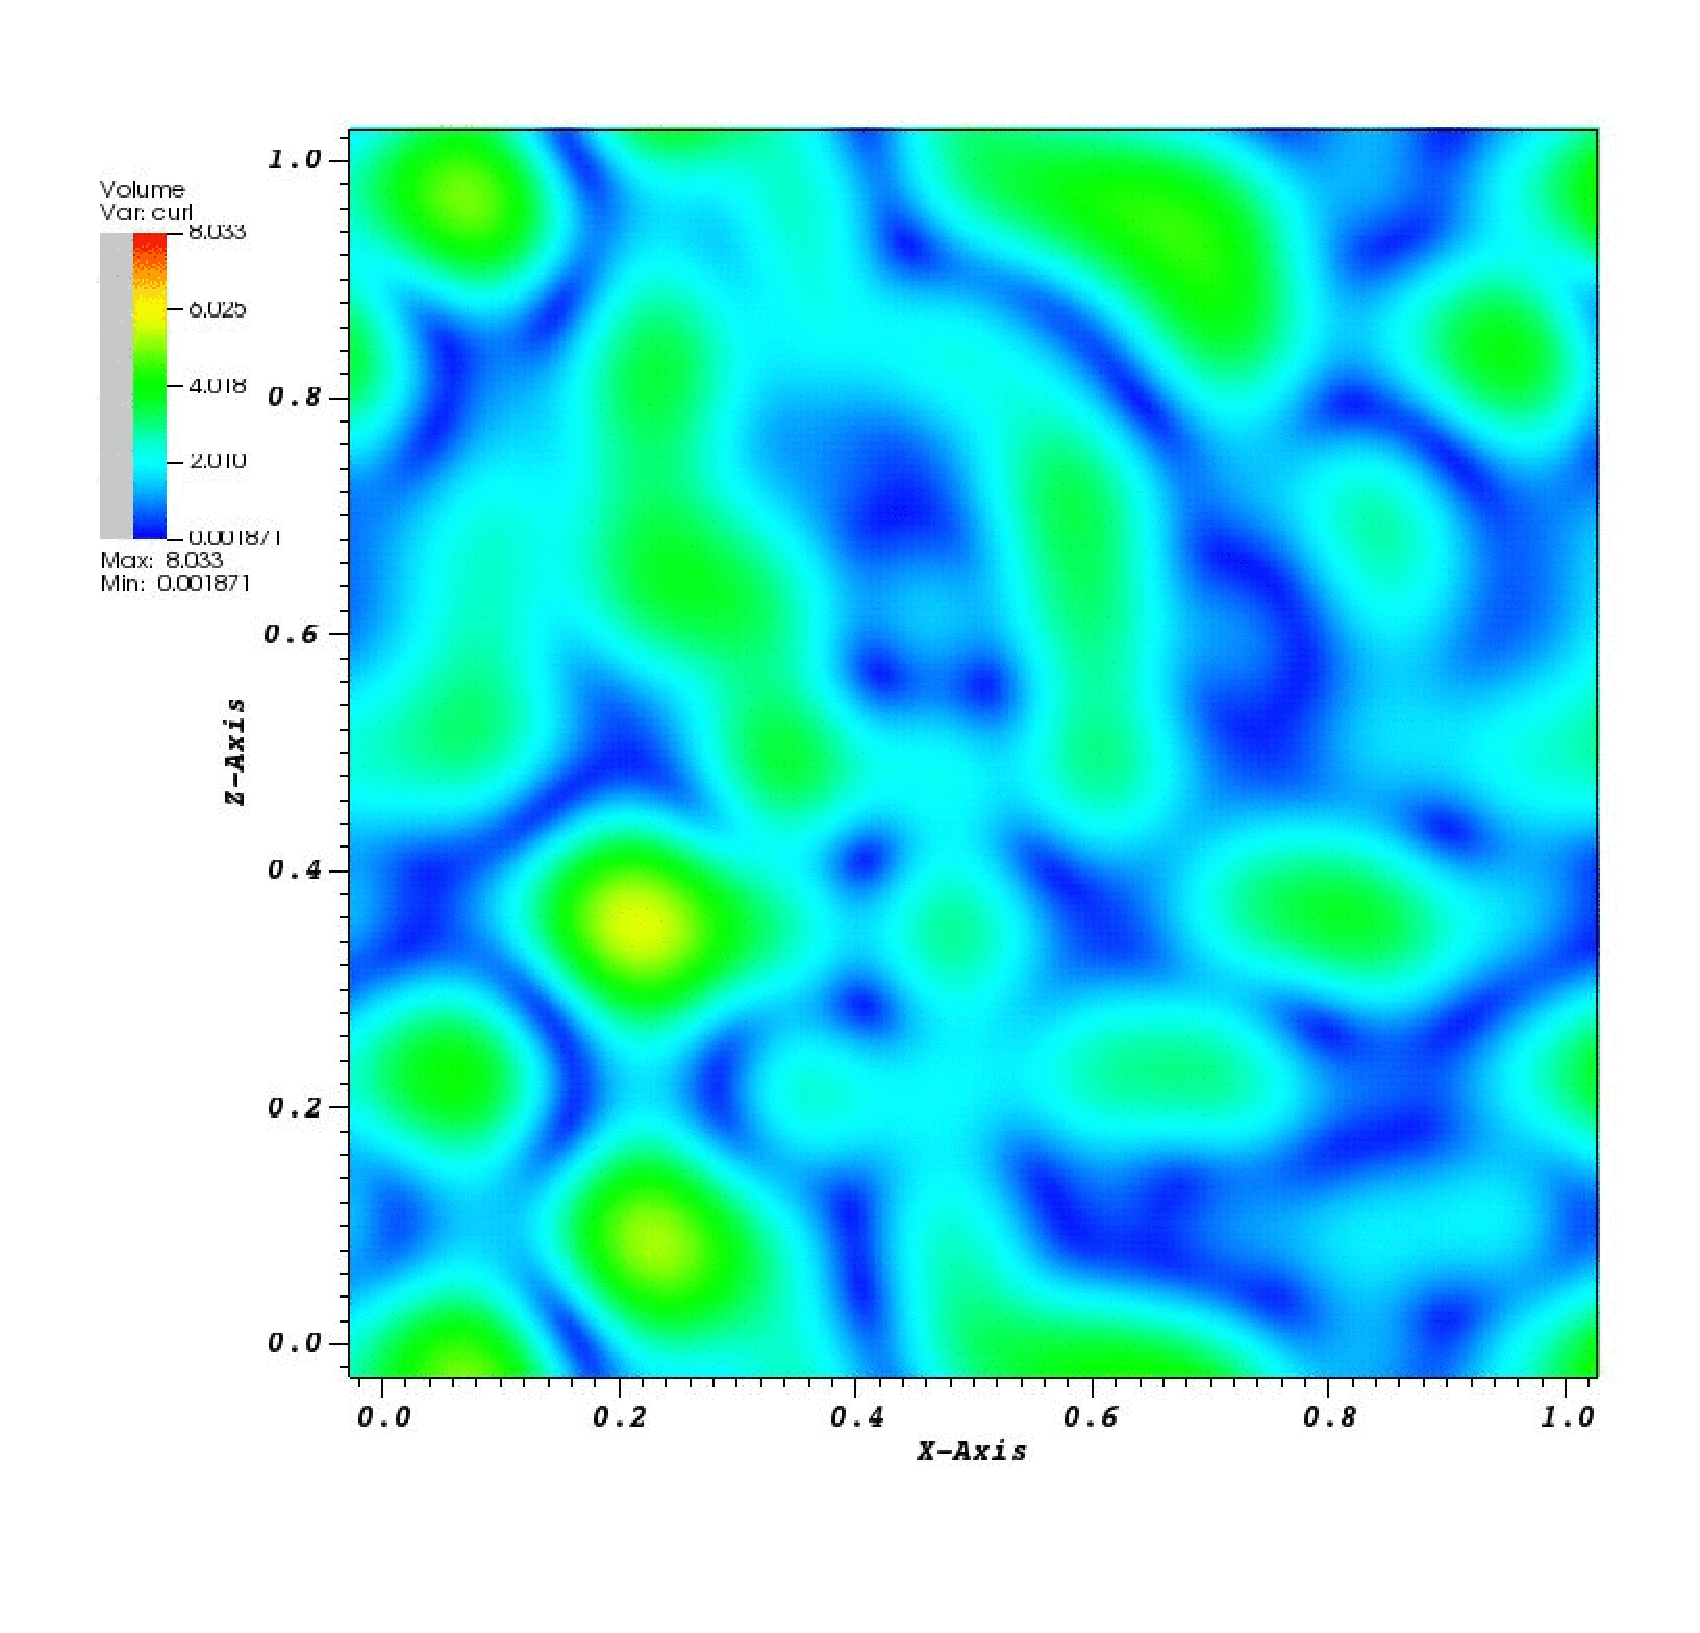
\includegraphics[width=0.48\textwidth]{Figures/vortex-0}
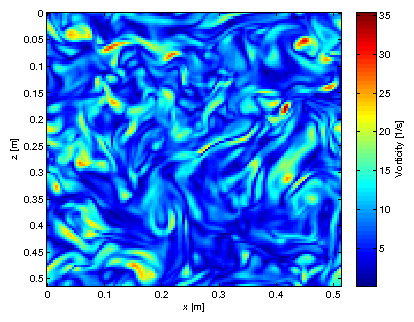
\includegraphics[width=0.48\textwidth]{Figures/vortex-1}

\caption{initial and final enstrophy field in x-z cross-sectional
plane defined as $\varepsilon(\mathbf{u}) = 0.5(\nabla\times\mathbf{u})^2$\label{fig:enstrophy}}
\end{figure}

\subsection{Initial vapor mixing ratio and temperature}
A straightforward way to initialize the vapor mixing ratio is to divide the computational domain into the regions of cloudy and clear air, then assign different values to each subdomain. By specifying the initialization functions, various initial profile for the vapor mixing ratio can be achieved. For example, in \cite{And04}, the function is defined according to the sign of the velocity function in physics space. This configuration will be referred to as case 1. In \cite{Kumar11}, the author used an artificial continuous function to construct a slab-like cloud filament. This situation can also be approximated by a simple discontinuous function and will be referred to as case 2. Rotating the slab-like cloud clockwise by $90$ degree, we obtain case 3. The initial vapor content profile for three cases are given by equations (\ref{case1}--\ref{case3}) and illustrated in figure (\ref{fig:v_field_case123}).
\begin{equation}
\mbox{case 1: } q_v(\mathbf{x},t=0) = 
\begin{cases} 
q_v^{max}, & u(\mathbf{x}) > 0\\
q_{v,e}, & u(\mathbf{x}) \le 0
\end{cases}\label{case1}
\end{equation}

\begin{equation}
\mbox{case 2: } q_v(x,t=0) = 
\begin{cases} 
q_v^{max}, & (L-d)/2 \le x < (L+d)/2\\
q_{v,e}, & \mbox{elsewhere}
\end{cases}\label{case2}
\end{equation}

\begin{equation}
\mbox{case 3: } q_v(z,t=0) = 
\begin{cases} 
q_v^{max}, & (L-d)/2 \le z < (L+d)/2\\
q_{v,e}, & \mbox{elsewhere}
\end{cases}\label{case3}
\end{equation}
where $q_v^{max}$ is maximum amplitude of $q_v$, which exceeds $q_{v,s}$ by $2\%$, and $q_{v,e}$ is the vapor mixing ratio of the clear air. $L$ is the length of computational domain, and $d = L/2$ is the width of the cloud slab. The $q_{max}$ in each case is set to be $3.95g/kg$ and the $q_{v,e}$ is $0.03g/kg$. The simulation is terminated when droplets completely evaporate or the supersaturation field becomes nearly uniform ($std<0.0002$).
\begin{figure}[H]
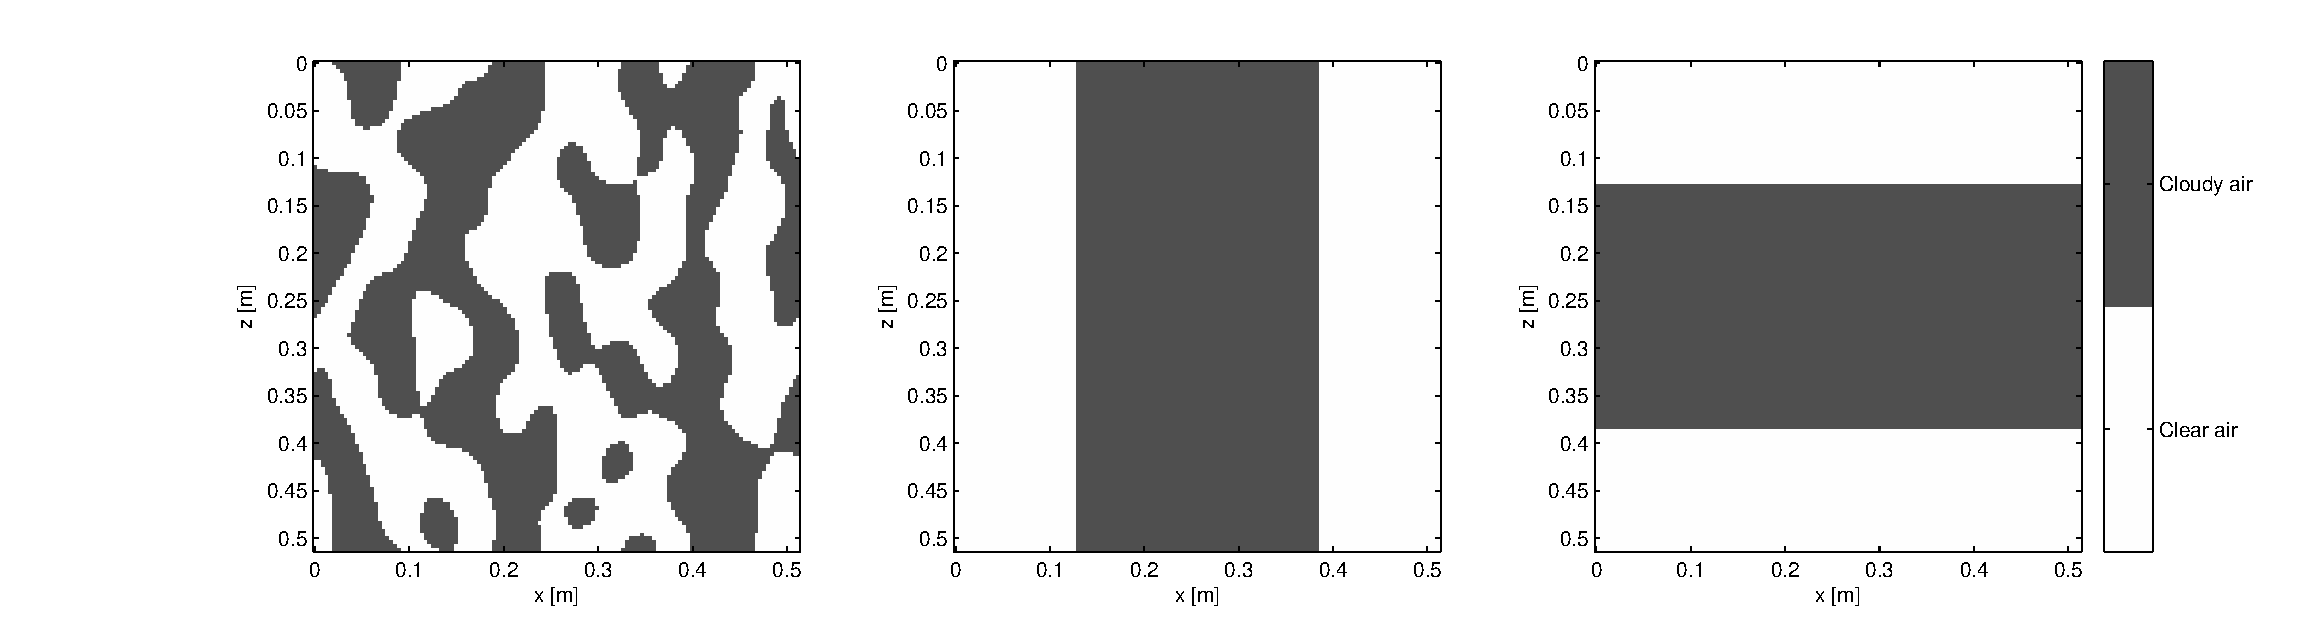
\includegraphics[width=1.0\textwidth]{Figures/v_field_case123}
\caption{Cross sectional view of the initial vapor mixing ratio for different cases: case 1, 2, 3 from left to right. The cloudy part occupies about half of the computational domain.\label{fig:v_field_case123}}
\end{figure}

Finally, the temperature field is initialized by imposing the neutral buoyancy restriction:
\begin{equation}
T(x,t = 0) = T_0 - 0.608T_0[q_v(x,t = 0) - q_{v0}]
\end{equation}
where the reference values are defined by volume averages $T_0 = \langle T(t=0)\rangle_V$ and $q_{v0} = \langle q_v(t=0)\rangle_V$. This condition implies that neither the vapor mixing ratio nor temperature would contribute to the initial buoyancy. This procedure is only performed for the initial temperature field and will completely follow \Eq{eq:Temp} afterwards.
\subsection{Initial droplets}

The cloud water is distributed to approximately $10^{7}$ number of droplets, which have the same sizes and are uniformly placed in the cloudy region at time $0s$. \textcolor{red}{how to decide?} After the turbulence reaches a steady state in a short time, the droplets will be freed to move and change their sizes according to the physics law. A droplet with zero radius will be immediately removed from the computational domain and will not contribute to any statistical results. Some important quantities for initial condition are summarized in \Table{tb:parameters}.

\begin{table*}
\begin{tabular}{l c c c c c}
\hline\hline
Quantity & Symbol & Value & Quantity & Symbol & Value\\
\hline
Grid points & $N$ & $256$ & Droplet radius & $R_{0}$ & $15\mu m$\\
Box length & $L$ & $0.512m$ & Environ supersat & $S_{e}$ & $-0.99$\\
Grid size & $a$ & $0.002m$ & Cloud supersat & $S_{c}$ & $0.02$\\
Viscosity & $\nu$ & $1.5\times10^{-5}m^{2}s^{-1}$ & Number density& $N_{c}$ & $153cm^{-3}$\\
Dissip rate& $\epsilon$ & $2.0\times10^{-3}m^{2}s^{-3}$ & Eddy turnover time & $\tau_{L}$ & $4.27s$\\
Dissip length& $\eta$ & $10^{-3}m$ & Evaporation time & $\tau_{evap}$ & $2.09s$\\
Dissip time& $\tau_{\eta}$ & $0.087s$ & Reaction time & $\tau_{react}$ & $6.36s$\\
\hline
\end{tabular}
\caption{Initial conditions}
\label{tb:parameters}
\end{table*}

\section{Numerical Results}
The main goal in this paper is using numerical simulation to study
the entrainment and mixing process which often occurs near the cloud-clear air interface. In this section, some principal results are presented, including thermodynamics, microphysics.

\subsection{Thermodynamics}
In \Fig{fig:therm_dynam}, we inspect different cases by comparing the behaviors of their macroscopic 
variables: the temporal evolution of the turbulent kinetic energy (a), droplets number concentration (b), standard deviation and relative dispersion of temperature (c,d) and the same for water vapor mixing ratio (e,f). 

In panel (a), the turbulent kinetic energy (TKE) of the forced cases F1, F2 and F3 remains on average after a short relaxation at the initial time. However, it is interesting to observe a transient growth in the decaying cases before continuing to decay to zero. We interpret this growth as the results of buoyancy effect, which is caused by the deviation of temperature and vapor mixing ratio to the reference value according to \Eq{eq:source_term}. In details, case D1 could be regarded as the intermediate stage of mixing process in D2 or D3, therefore this deviation quickly disappear and show no growth in the figure. As for D2, the mixing only happens at the interface between cloudy and clear air, thus it takes much longer to damp the transient growth. The mixing in case D3 is accelerated by sedimentation effect, making it a little faster than D2.

The droplets number concentration for different cases are displayed in panel (b). All cases have the same equilibrium state with a zero liquid water content. The rate at which droplets evaporate is higher for the forced turbulence than the decaying turbulence except D1. Since D1 has a complex structure of cloud filaments at the initial time, all the droplets will quickly be exposed to the same environment and begin to evaporate, leading to its number concentration curve to be similar as the forced cases.

Panel (c) and (d) show the standard deviation and relative dispersion of temperature field. In spite of similar configuration with D2, case D3 has a stronger growth in amplitude. We interpret this finding as a indication that the droplets movements are accelerated in the vertical direction by the sedimentation effect. Most of the droplets have a chance to enter into the clear air and evaporate at an early stage. This evaporation process will absorb latent heat from the environment thus strongly deviate the temperature field from the mean value. However, this difference becomes smaller in the forced turbulence as the motion of particles is almost dominated by the external forcing which are the same for F1, F2 and F3.

Panel (e) and (f) present the standard deviation and relative dispersion of vapor mixing ratio. In these figures, we cannot observe any transient growth as shown for temperature field. This result is consistent with the ones in \cite{Kumar14}. Notice that the vapor mixing ratio in the clear air is much lower than in the cloudy air. The droplets entering into the clear region will quickly turn into the vapor while the droplets staying in the cloudy region continue to condensate. This phase transition process will reduce the difference of vapor mixing ratio between clear air and cloudy air, thus the transient growth of the deviation could not be observed.

\begin{figure}\centering
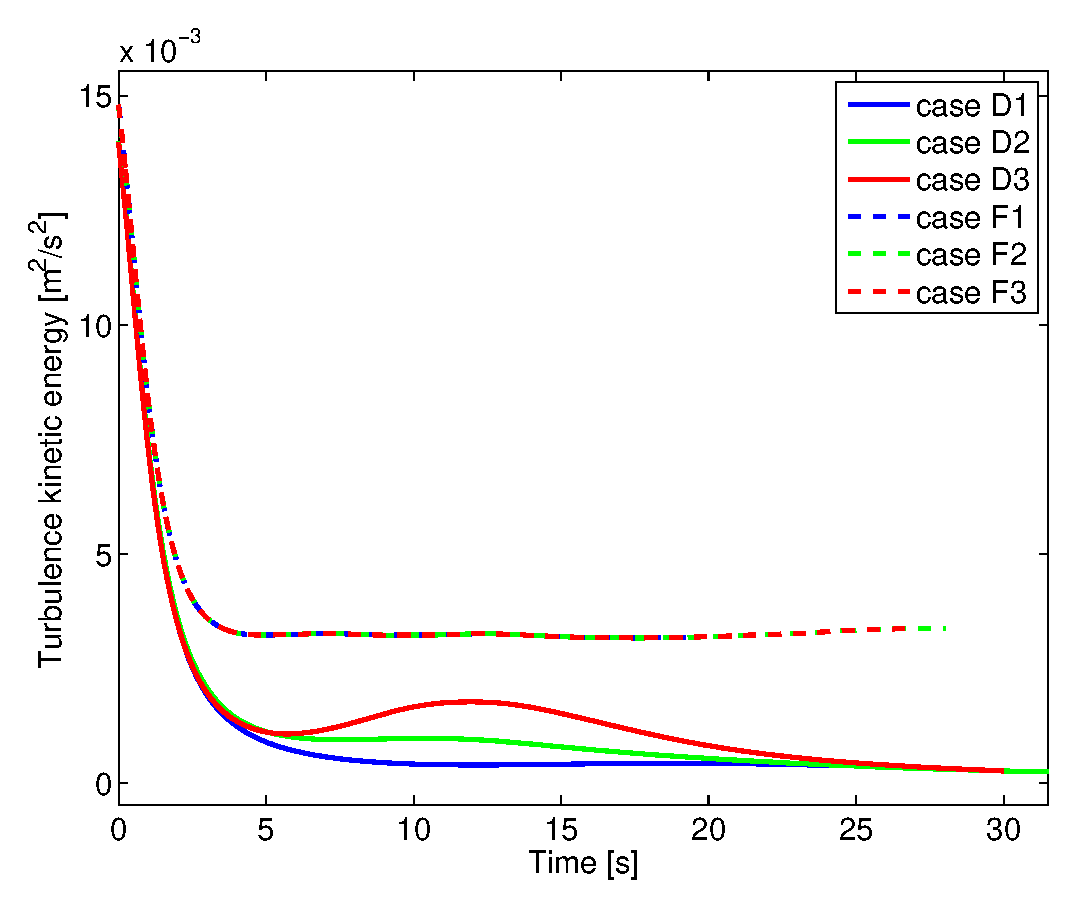
\includegraphics[width=0.48\textwidth]{Figures/tke}
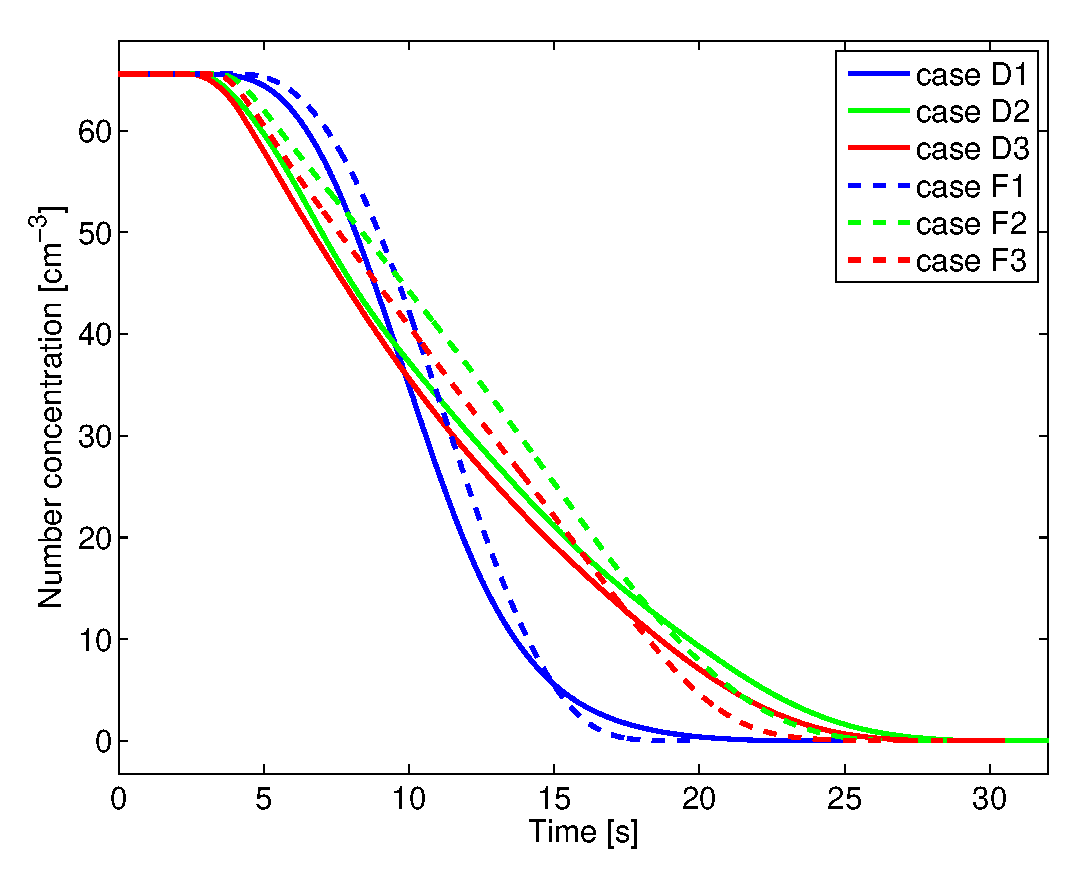
\includegraphics[width=0.48\textwidth]{Figures/num_con}\\
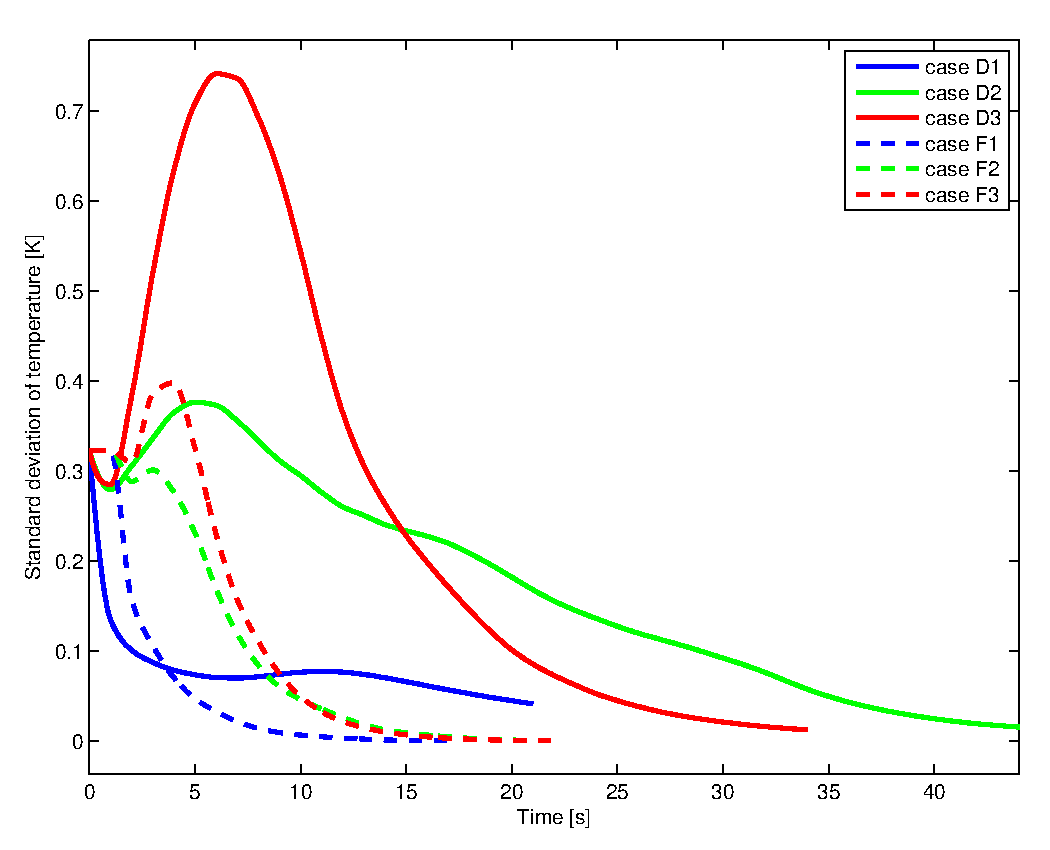
\includegraphics[width=0.48\textwidth]{Figures/temp_std}
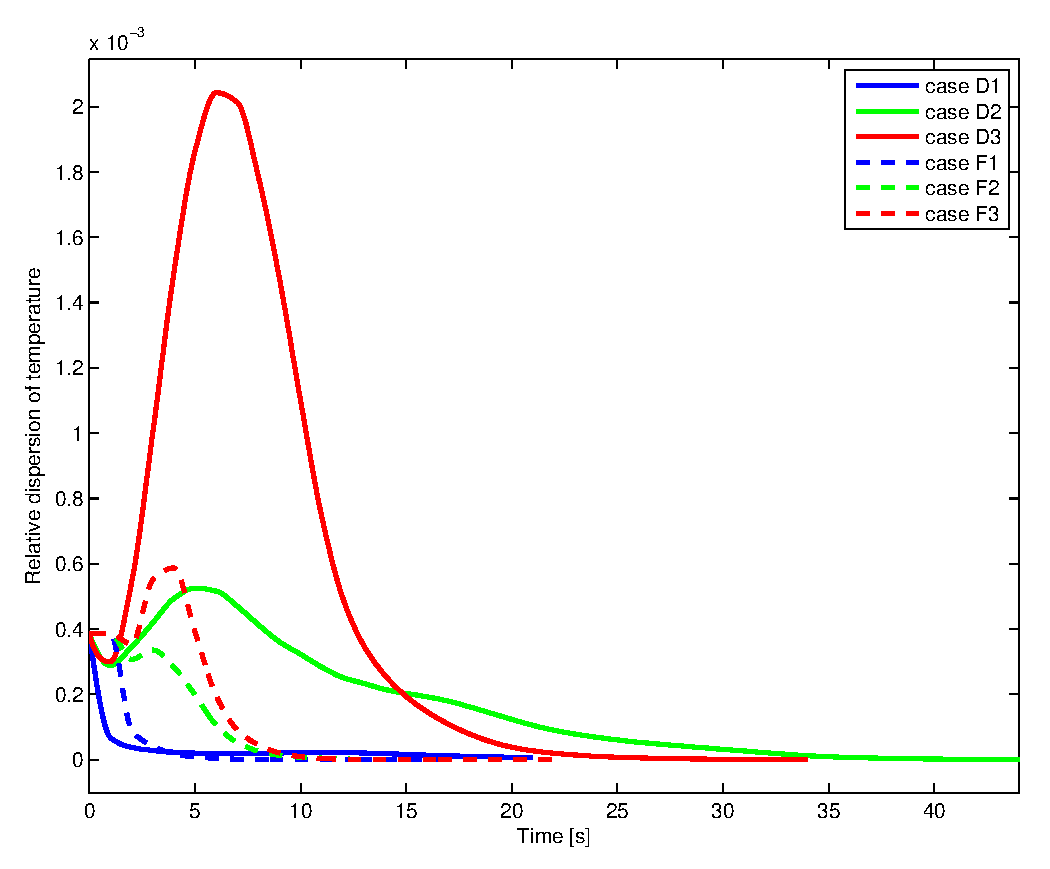
\includegraphics[width=0.48\textwidth]{Figures/temp_dsp}\\
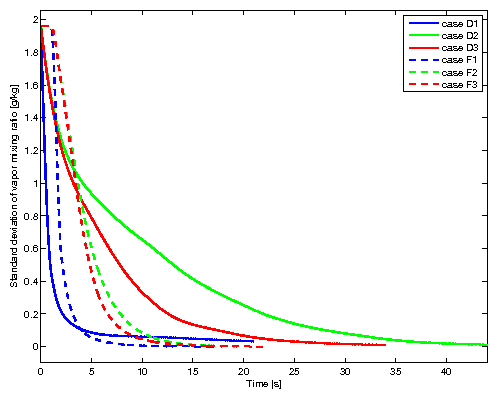
\includegraphics[width=0.48\textwidth]{Figures/vapor_std}
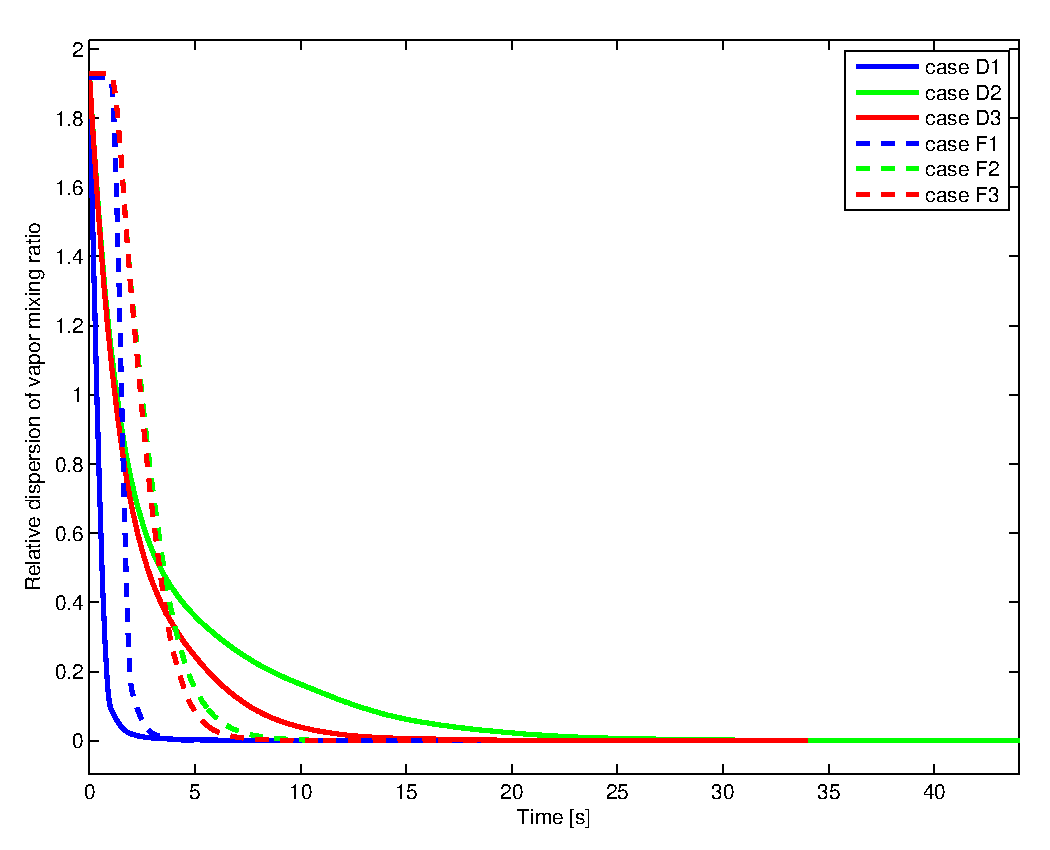
\includegraphics[width=0.48\textwidth]{Figures/vapor_dsp}
\caption{Thermodynamics of three cases, from left to right, up to bottom, are turbulence kinetic 
energy (a), droplets number concentration (b), standard deviation (c), relative dispersion (d) of temperature field and the same for the vapor mixing ratio (e,f).\label{fig:therm_dynam}}
\end{figure}

\subsection{Microphysics}
The radius distributions for case 1, 2 ,3 in both decaying and forced turbulence are displayed in \Fig{fig:rad_distri}. At the initial stage, some droplets enter into the clear air and expand their size distribution. As mixing going on, since the environment becomes unsaturated and homogeneous, the distribution starts to shift to zero. It continues approaching to zero until completely evaporation happens or the background environment becomes saturated. 
In the \Fig{fig:rad_distri}, an important observation is that case D1, D2 and D3 are quite different in both reaction time and size distribution. However, by substituting the buoyancy by external force, these difference almost disappear. This demonstrates that the difference is caused by the buoyancy term in \Eq{eq:source_term}. In specific, the buoyancy plays as a source of kinetic energy, so as to accelerate the motion of fluid field.
\begin{figure}[H]\centering
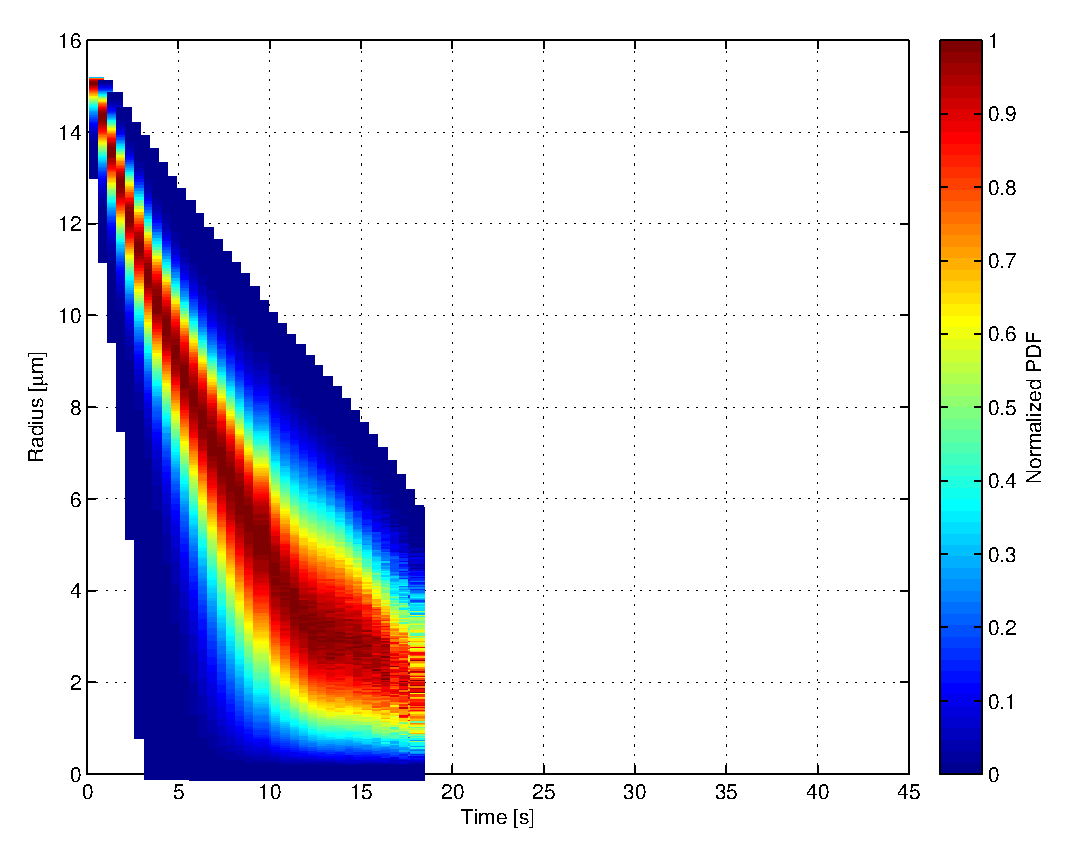
\includegraphics[width=0.48\textwidth]{Figures/pdf_radius_d1}
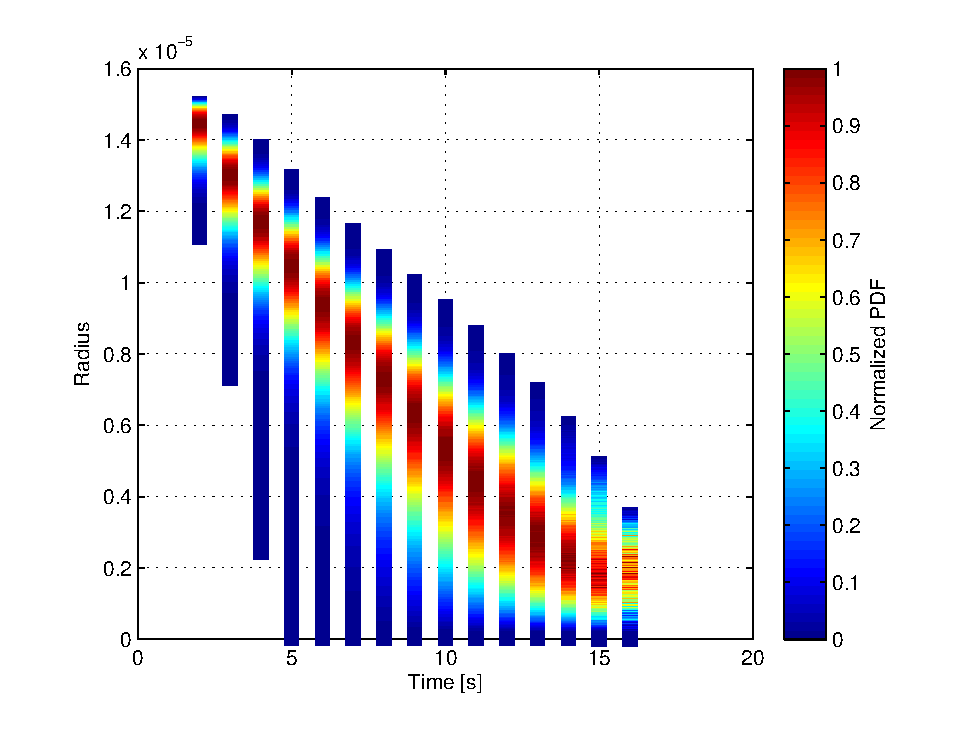
\includegraphics[width=0.48\textwidth]{Figures/pdf_radius_f1}\\
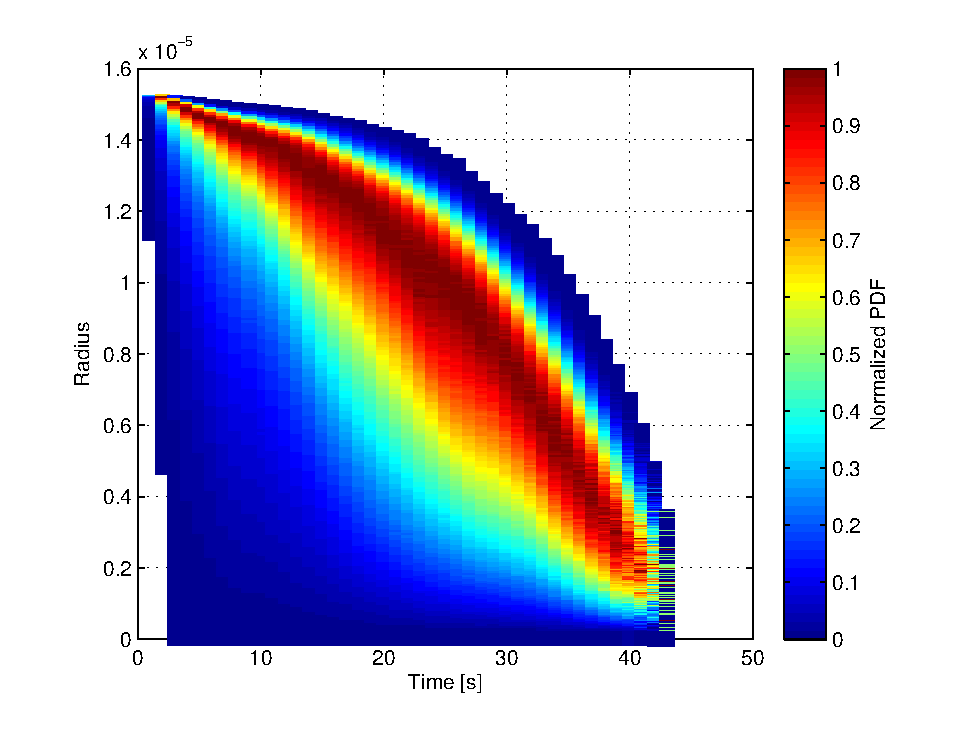
\includegraphics[width=0.48\textwidth]{Figures/pdf_radius_d2}
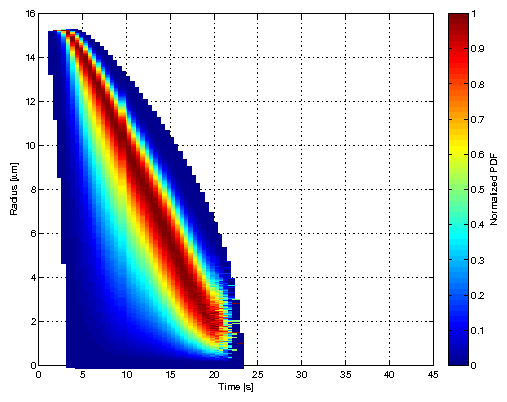
\includegraphics[width=0.48\textwidth]{Figures/pdf_radius_f2}\\
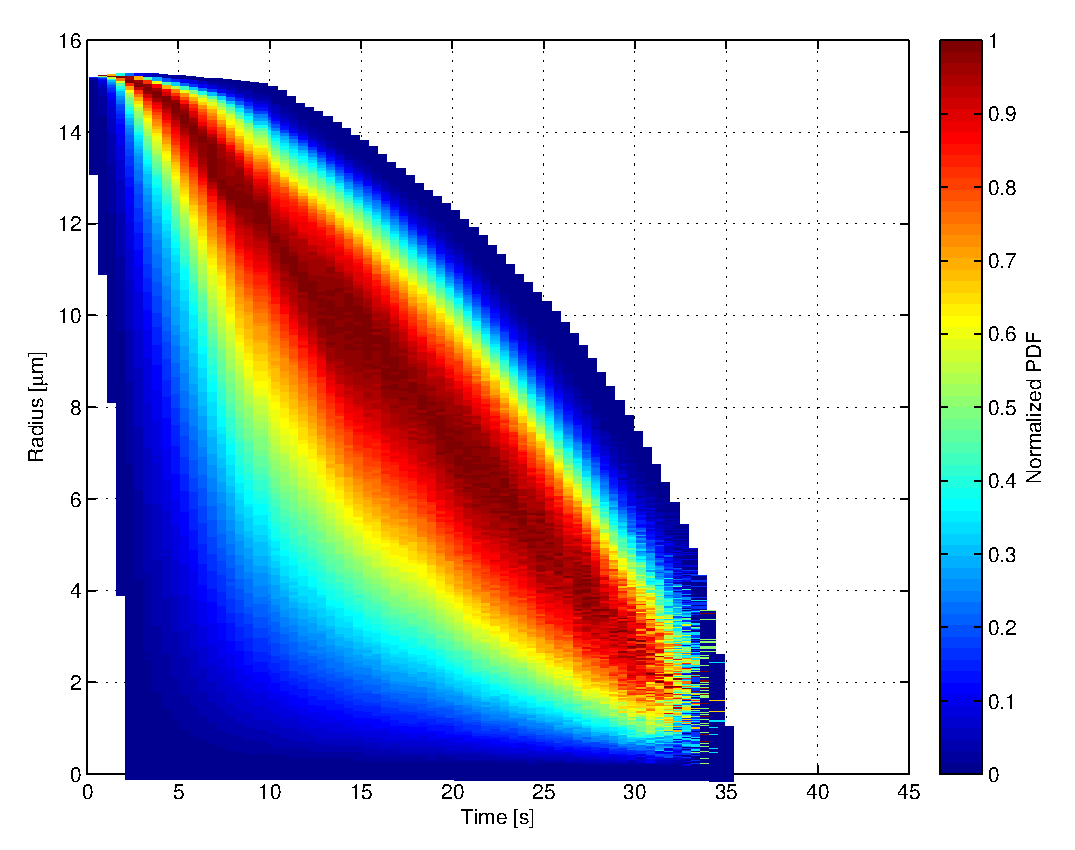
\includegraphics[width=0.48\textwidth]{Figures/pdf_radius_d3}
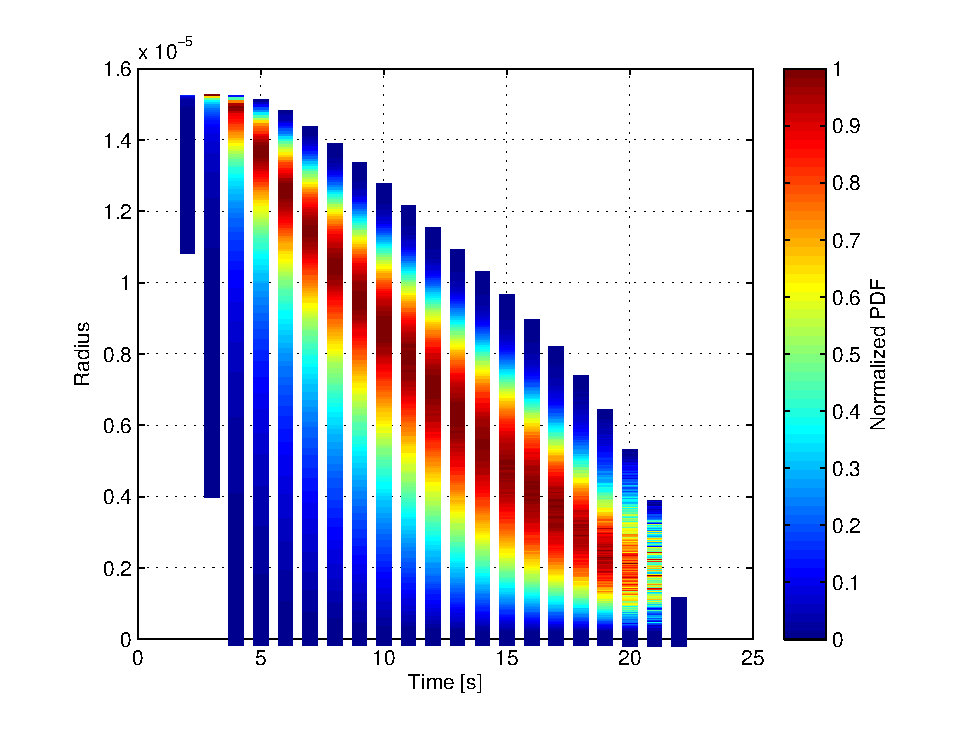
\includegraphics[width=0.48\textwidth]{Figures/pdf_radius_f3}
\caption{Evolution of radius distribution for decaying turbulence (left column) 
and forced turbulence (right column). From up to bottom are case 1, case 2 and case 3 respectively.}\label{fig:rad_distri}
\end{figure}

The distribution of supersaturation in \Fig{fig:supersat_distri} also clearly reflects the mixing process. Firstly, all the droplets stay in the cloud filaments thus has narrow spectrum and high probability density. After some droplets entering into the clear air, the spectrum immediately expands but with low probability density. This stage could be observed in D2 and D3, but extremely short for the rest cases. As mixing going on, the environment becomes much more homogeneous, that is most droplets stay in a similar environment. Finally, the environment becomes well-mixed, droplets completely evaporate and all the cases reach the same state.
\begin{figure}[H]\centering
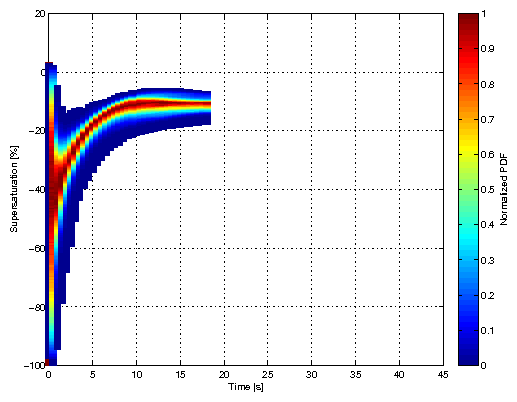
\includegraphics[width=0.48\textwidth]{Figures/pdf_supersat_d1}
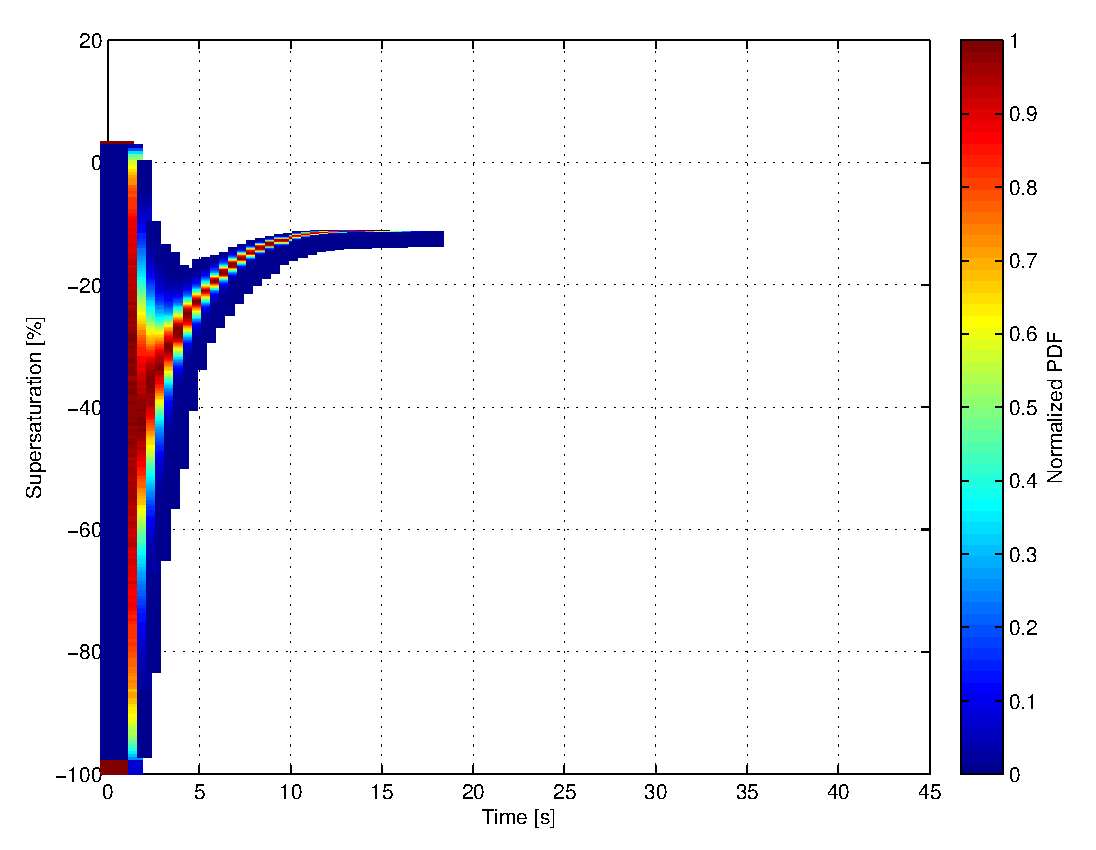
\includegraphics[width=0.48\textwidth]{Figures/pdf_supersat_f1}\\
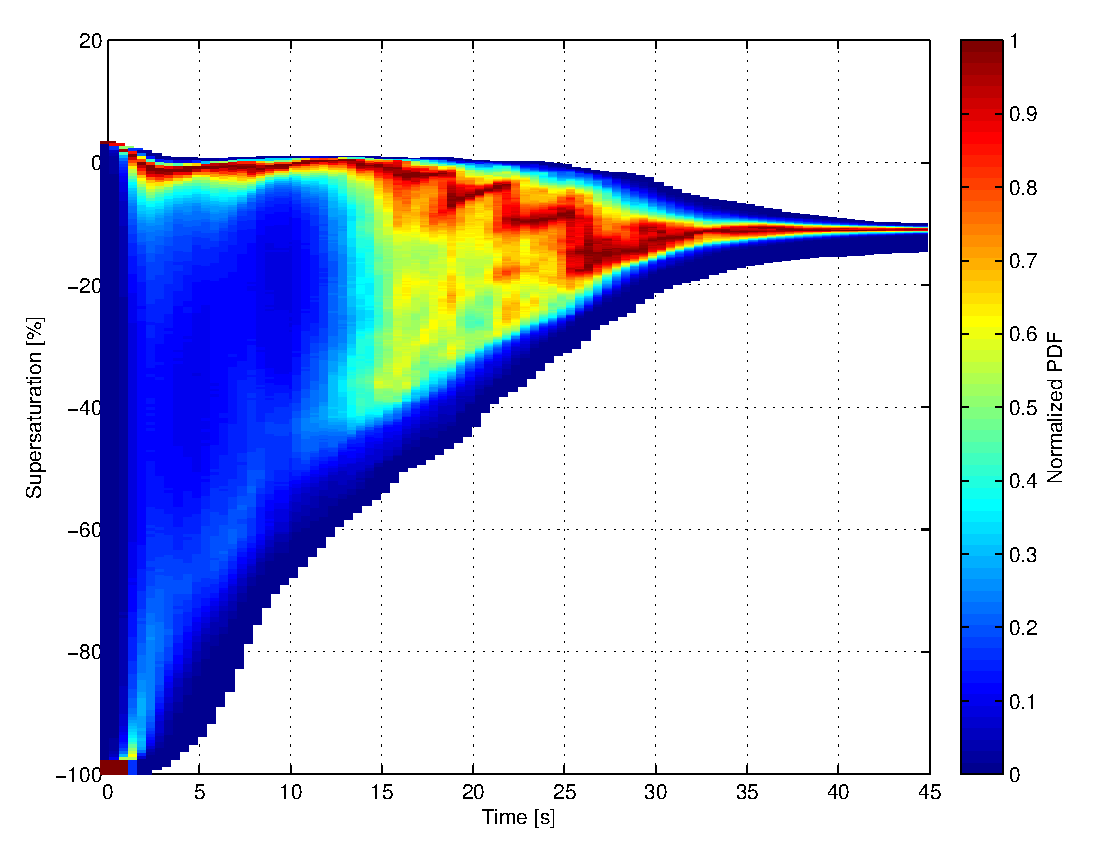
\includegraphics[width=0.48\textwidth]{Figures/pdf_supersat_d2}
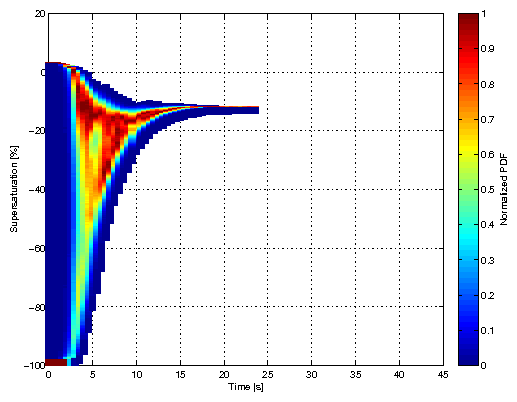
\includegraphics[width=0.48\textwidth]{Figures/pdf_supersat_f2}\\
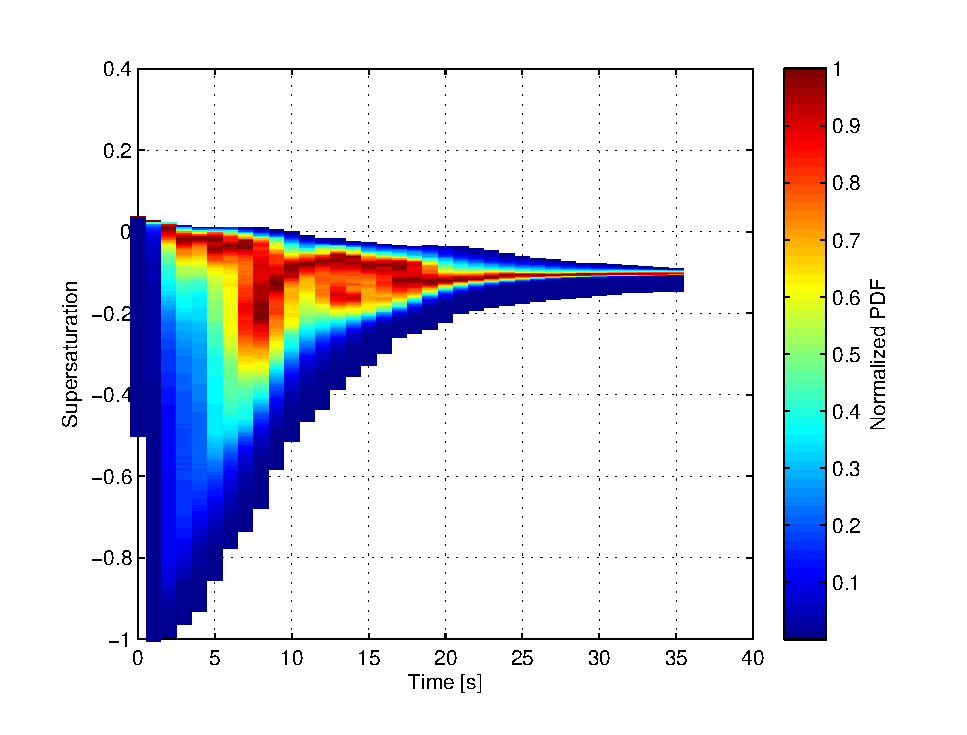
\includegraphics[width=0.48\textwidth]{Figures/pdf_supersat_d3}
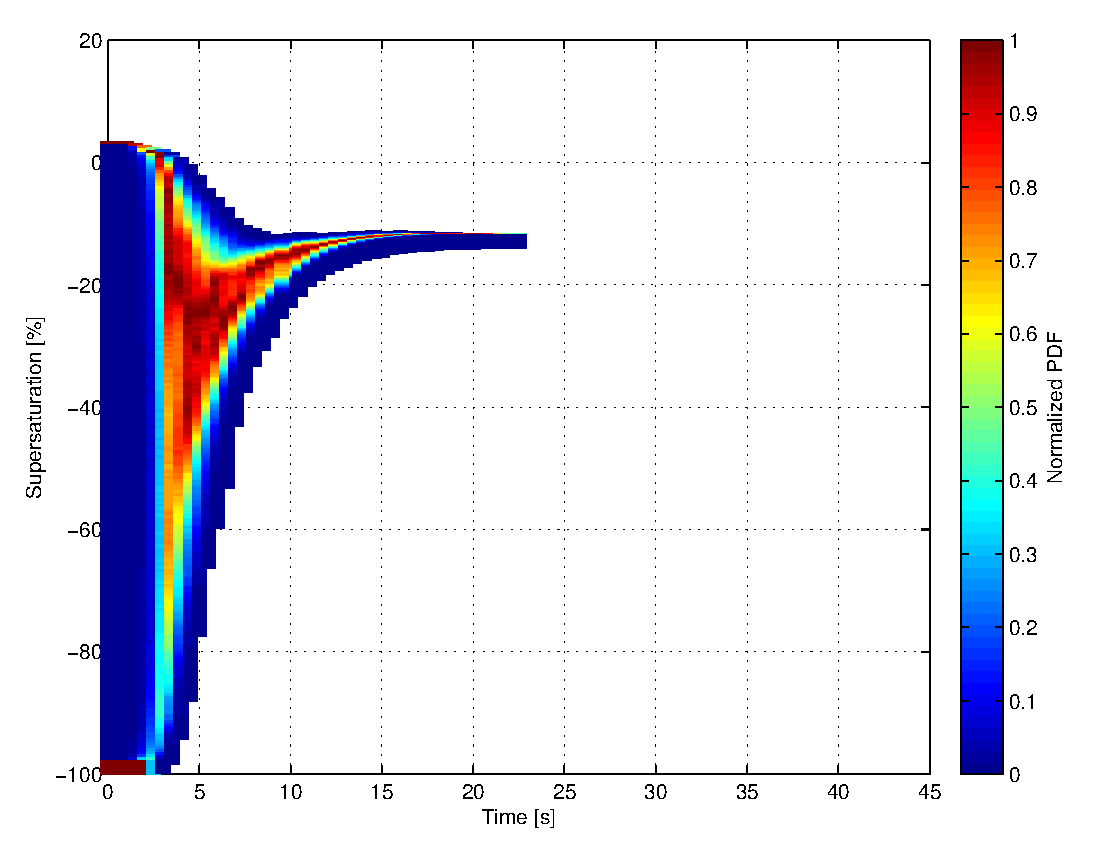
\includegraphics[width=0.48\textwidth]{Figures/pdf_supersat_f3}
\caption{Evolution of supersaturation distribution for decaying turbulence (left column) and forced turbulence (right column). From up to bottom are case 1, case 2 and case 3 respectively. In conclusion, the shape of the cloud filament has no influence on the final state after the mixing but will affect the intermediate process. The shape also has little impact on the mixing process for forced turbulence, while can not be completely ignored in the decaying cases. The results suggest that the initial shape of cloud filaments should be considered as an important factor when studying mixing scenario without external forcing.}\label{fig:supersat_distri}
\end{figure}

\section{Entrainment and mixing processes}
Depending on the mixing scenario (the homogeneity of mixing), the
droplets will evolve in quite different ways. In the extremely homogeneous mixing scenario, the number of droplets does not change while the mean radius decreases. In the extremely inhomogeneous mixing scenario, some droplets in the cloud completely disappear while the others remain unchanged. This mixing of clear and cloudy air is often quantified by the Damkohler number:

\begin{equation}
Da=\frac{\tau_{mix}}{\tau_{react}}\label{eq:DaNumber}
\end{equation}


here $\tau_{mix}$ is the time scale for an eddy of size $l_E$ and is defined as:

\begin{equation}
\tau_{mix}=(\frac{l_E^{2}}{\varepsilon})^{1/3}\label{eq:Tmix}
\end{equation}

$\tau_{react}$ is the time for complete chemical reaction, which often given by the evaporation time scale in the cloud physics literature:
\begin{equation}
\tau_{e}=\frac{R_{m}^{2}}{-KS}\label{eq:Tevap}
\end{equation}
where $R_{m}$ is the mean radius of a droplets group and $K$ is defined
by (\ref{eq:CondCoeff}), $S$ is the averaged supersaturation over
the cloud-free part of the computational domain. In general, $Da\ll1$ corresponds to the homogeneous mixing while $Da\gg1$ is the inhomogeneous one. The real entrainment and mixing process has a $Da$ number often between
these two limits.

The $\tau_{react}$ is computed by solving the following ordinary differential equation with instantaneous volume mean radius and mean supersaturation as the initial condition:
\begin{equation}
\frac{dR_{m}}{dt}=K\frac{S}{R_{m}}\label{eq:DiffR}
\end{equation}

\begin{equation}
\frac{dS}{dt}=-BR_{m}S\label{eq:DiffSuper}
\end{equation}
where $B$ is a function of pressure and temperature, whose specific definition can be found in \cite{Chunsong11}. In spite of popularity, this approach has a shortcoming:
the value of $l_E$ used in (\ref{eq:Tmix}) is ambiguous. To overcome this difficulty, Lehmann(\cite{Lehmann09}) introduced the concept of transition length $l^{*}$, at which the mixing transits from inhomogeneous to homogeneous:
\begin{equation}
l^{*}=\varepsilon^{1/2}\tau_{react}^{3/2}\label{eq:TransL}
\end{equation}
where the reaction time $\tau_{react}$ is defined as either the time when the droplets have completely evaporated or the time at which the averaged supersaturation $S>-0.005$. 
With transition length $l^{*}$, a dimensionless number called transition scale number was introduced in \cite{Chunsong13} and defined as the ratio of $l^{*}$ and Kolmogorov length scale $\eta$:

\begin{equation}
N_{L}=\frac{l^{*}}{\eta}\label{eq:NL}
\end{equation}

To characterize the microphysical properties of the mixing, the $\langle r^3\rangle -N_d$ diagram (volume mean radius versus number density) was introduced in \cite{Burnet07} and has been widely applied to study the homogeneous/inhomogeneous entrainment-mixing process. With $\langle r^3\rangle -N_d$ diagram, one can predict the extremely homogeneous mixing line at different supersaturation (\cite{Lehmann09,Kumar14}). An useful quantity is the homogeneous mixing degree $\alpha$:

\begin{equation}
N=N_{a}(\frac{q_l}{q_{l_0}})^{\alpha}\label{eq:alpha}
\end{equation}
where $N_{a}$ and $q_{l_a}$ are the adiabatic value of number density and liquid water mixing ratio, and $N$ and $q_{l}$ are the instantaneous values in the sample boxes. Lu et. al. (2012, 2015) introduced other microphysical measures to quantify different mixing mechanisms.

Following \cite{Kumar14}'s idea, the computational domain is divided into $64$ equal-sized sample boxes. We keep tracking the volume mean radius and number concentration for each sample box and make them scaled by the adiabatic values. The mixing diagram for different cases are displayed in \Fig{fig:mixing_diagram}. In the mixing diagram, the homogeneous mixing line (red dotted) and inhomogeneous mixing line (black dotted) are plotted in the diagram for reference. 

In the top panel, the mixing diagram of D1 and F1 does not start from the $(1,1)$ point since the initial droplets in a sample box have already been diluted and the their number concentration are much less than the adiabatic value. The droplets number concentration remains nearly unchanged until some droplets completely evaporate. As claimed in \cite{And04}, this configuration excludes the dilution effects and can only be used to simulate the final stage of the entrainment and mixing process. The difference between forced turbulence and decaying turbulence is not obvious.

In the middle panel, the mixing diagram shows the mixing curves for case D2 and F2. As the observation in \cite{Kumar14}, the inhomogeneous offset could be also be observed in panel (c) and (d).
\begin{figure}\centering
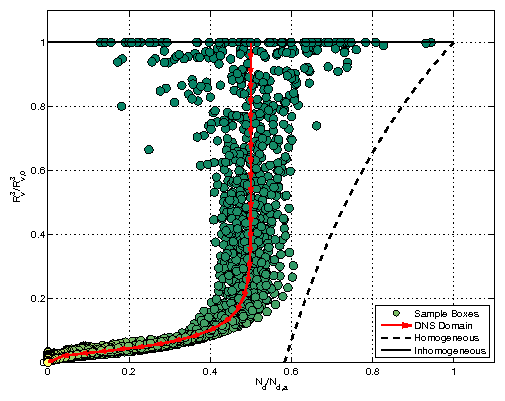
\includegraphics[width=0.48\textwidth]{Figures/mixing_cased1}
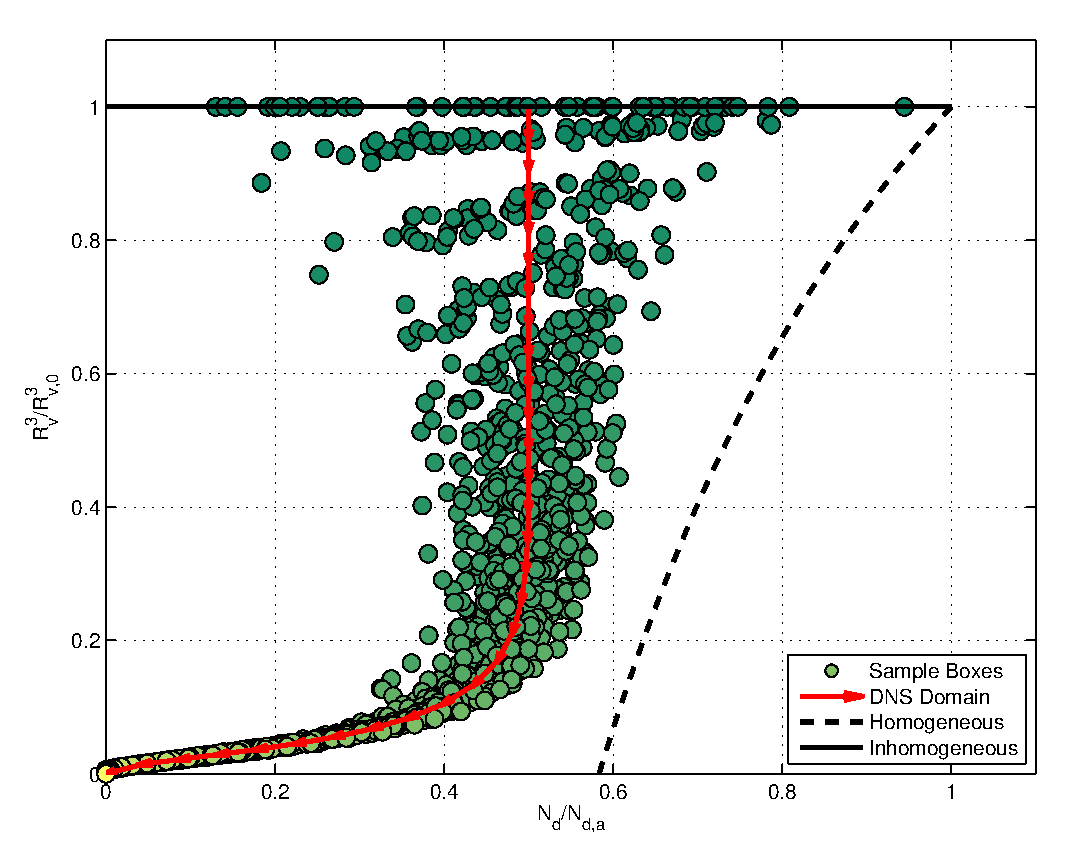
\includegraphics[width=0.48\textwidth]{Figures/mixing_casef1}\\
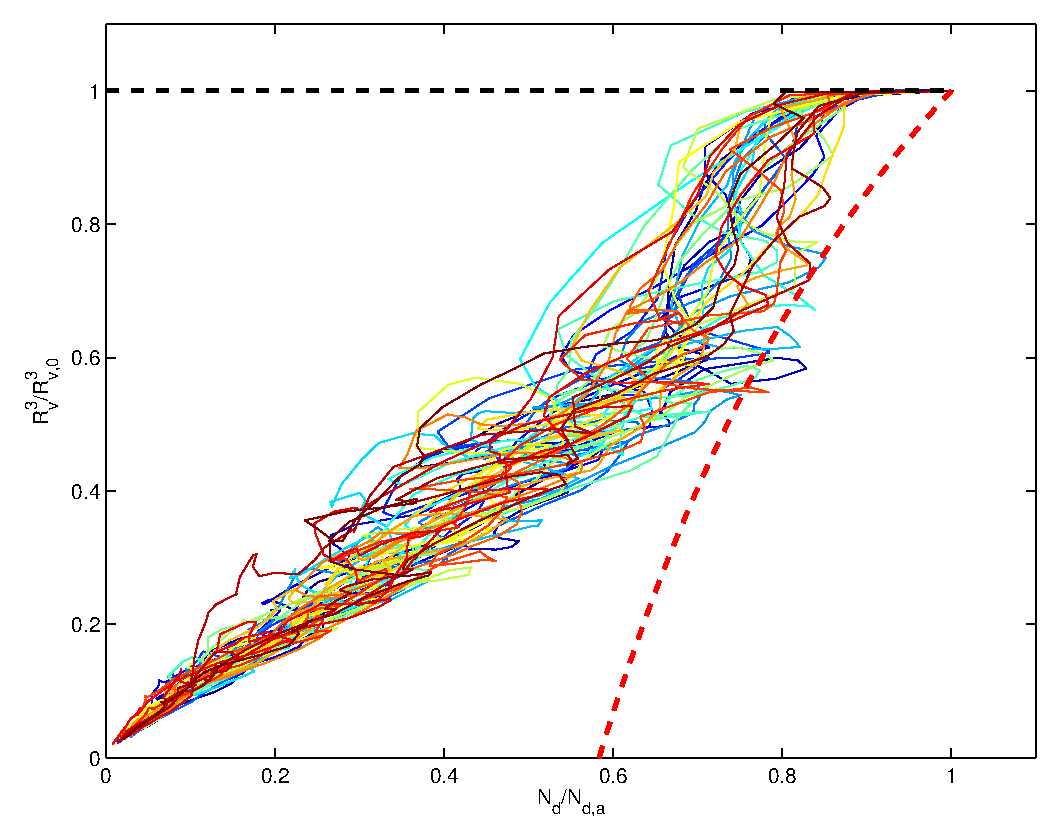
\includegraphics[width=0.48\textwidth]{Figures/mixing_cased2}
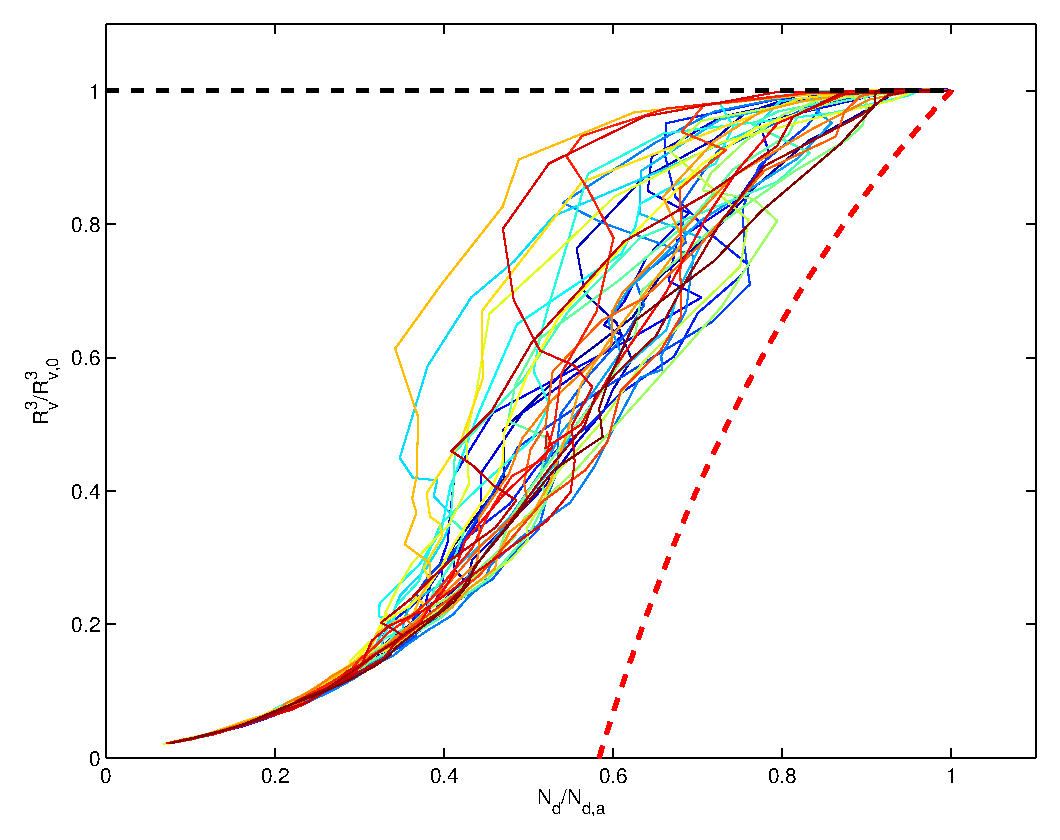
\includegraphics[width=0.48\textwidth]{Figures/mixing_casef2}\\
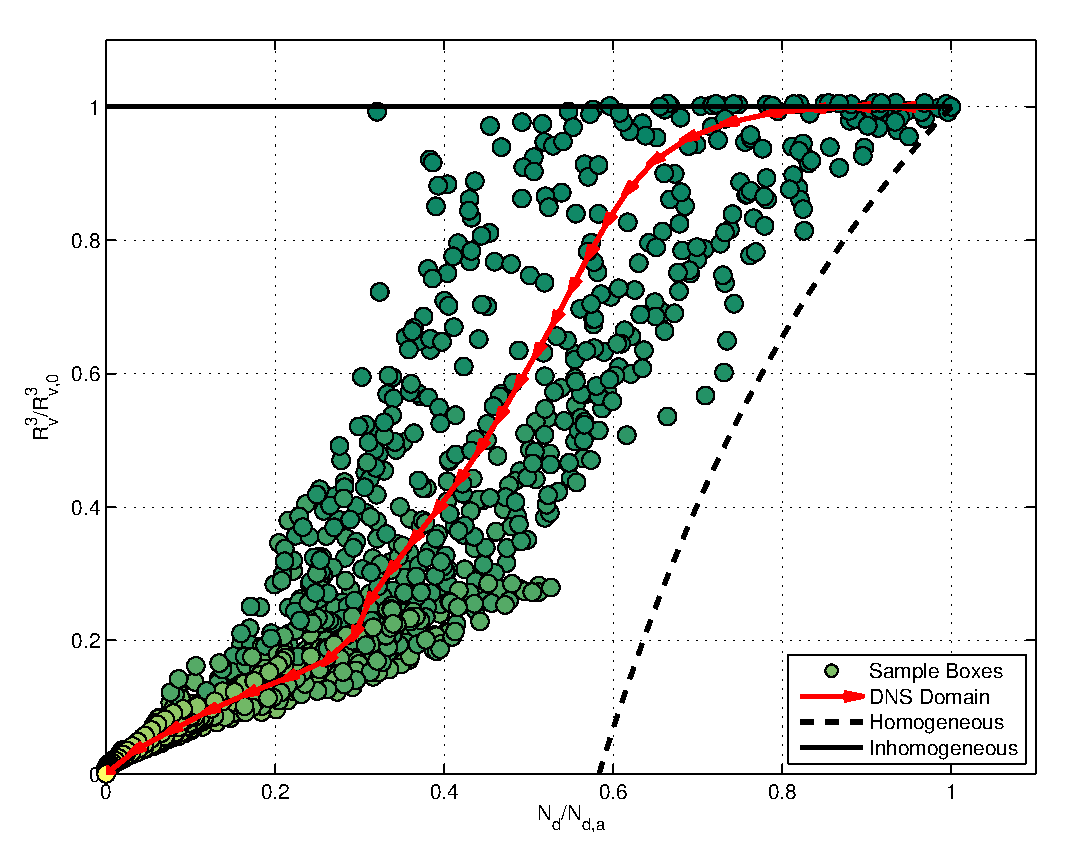
\includegraphics[width=0.48\textwidth]{Figures/mixing_cased3}
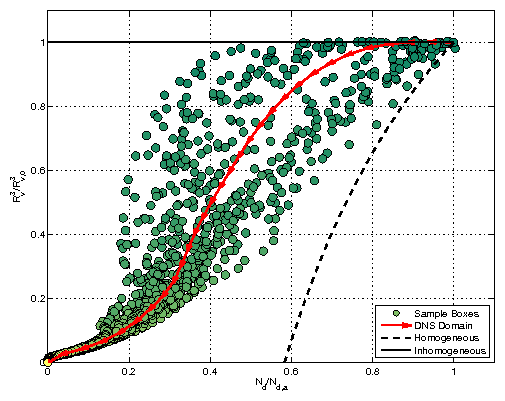
\includegraphics[width=0.48\textwidth]{Figures/mixing_casef3}
\caption{Mixing diagram for case D1, D2, D3, F1, F2 and F3. Mean cubic radius and mixing fraction have been calculated in 64 equal-sized samples boxes. Only the boxes with non-zero particles at the initial time will be counted.\label{mixing_diagram}}
\end{figure}

\section{Effects of sedimentation on preferential concentration }
Clustering of inertial particles has been extensively studied via both 
experiments and numerical simulations \cite{Sundaram97, Reade2000}, but the sedimentation effects on the clustering are poorly understood. In this section, a series of numerical test are performed by gradually increasing the gravity force and calculate the corresponding clustering index \cite{Vaillancourt02} with
\begin{equation}
C_L = \hat{V}_L(n)/V_L(n)-1
\label{eq:cluster_index}
\end{equation}
where $\hat{V}_L(n)$ is the measured variance of the number density and $V_L(n)$ is the mean concentration of droplets.
From the history of the clustering index \Fig{fig:gravity_cluster}, one can clearly tell that the clustering index increase at the beginning stage due to the strong turbulence fluctuation and then decrease as the turbulence decaying. Another observation is that strong gravity force leads to weak preferential concentration results. The conclusion also holds for the forced turbulence. 
\textcolor{red}{
[(1) as suggested earlier, have a plot showing cluster index as a function of gravity; (2) to see the connection with preferential concentration, plot clustering index for different sized particles and droplet concentration of different sizes as a function of vorticity).
}
\begin{figure}[H]\centering
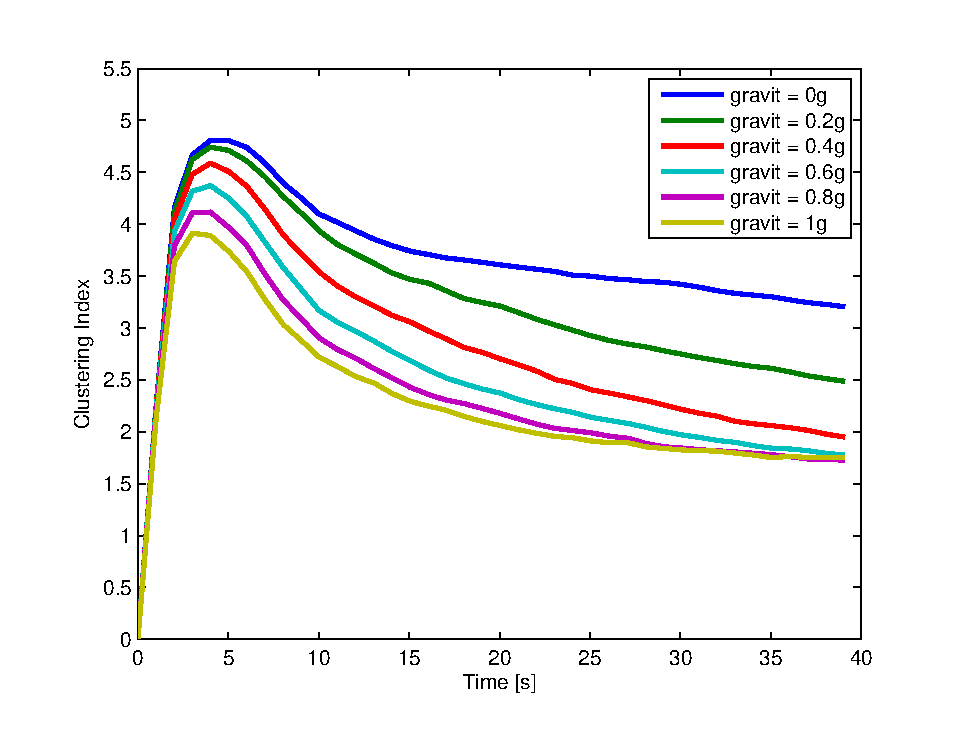
\includegraphics[width=0.45\textwidth]{Figures/gravity_time_decay}
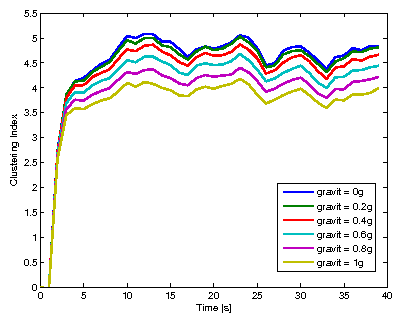
\includegraphics[width=0.45\textwidth]{Figures/gravity_time_force}
\caption{Time evolution of clustering index with different sedimentation term in decaying turbulence (see left) and 
forced turbulence (see right figure).}
\label{fig:gravity_cluster}
\end{figure}

\bibliographystyle{agufull08}
\bibliography{refs}

\end{article}
\end{document}
